\section{Einleitung}
Die wissenschaftliche Forschung wurde als wichtiger Einflussfaktor für die Entstehung neuer Technologien und Technologietrends in bedeutenden Studien nachgewiesen.\footcite[Vgl.][S.~187]{Nelson1986}\footcite[Vgl.][S.~11]{Mansfield1991}\footcite[Vgl.][S.~599]{Tegarden2012} Nach Jaffe wird diese Erkenntnis bereits durch die geographische Nähe von Zentren der Spitzentechnologie wie das "`Silicon Valley"' oder die "`Massachusetts Route 128"' zu führenden Universitäten gestützt.\footcite[Vgl.][S.~967f]{Jaffe1989} Nach einer Studie von Mansfield wären etwa 11~\% aller Produkte einer Auswahl aus sieben Fertigungsindustrien im Betrachtungszeitraum gar nicht oder nur mit erheblicher Zeitverzögerung entwickelt worden, wäre dem nicht eine entsprechende wissenschaftliche Forschung vorausgegangen.\footcite[Vgl.][S.~2]{Mansfield1991}

Dennoch liegt die maßgebliche Entscheidung über den Einsatz und die Weiterentwicklung neuer Technologien vorwiegend in Händen von Unternehmern, Managern und sonstigen Entscheidungsträgern der praktizierenden Wirtschaft. Die wiederum richten ihre Entscheidungen unter Berücksichtigung einer Vielzahl von Faktoren an den Markt aus, um den Unternehmenserfolg zu steigern.\footcite[Vgl.][S.~1652f]{Gruber2008} Dabei greifen sie auch auf Informationsquellen von spezialisierten Unternehmen zurück, die mit Hilfe proprietärer Methoden Prognosen für Technologietrends in eigenen Publikationen herausgeben. Einer der einflussreichsten und bekanntesten Vertreter dessen ist der "`Gartner Hype Cycle"', den große Unternehmen bei strategischen Entscheidungen bezüglich neuer Technologien beratend hinzuziehen.\footcite[Vgl.][S.~254]{Steinert2010}

Nach Beyer ist der Einfluss auf Technologietrends durch Wirtschaftsmedien höher als durch wissenschaftliche Artikel, da sie von Managern aufgrund des gewohnten Fachjargons sowie der Praxisrelevanz bevorzugt gelesen werden.\footcite[Vgl.][S.~472]{Beyer1992} Barley et al. fanden sogar heraus, dass sich gängige Begriffe der Wirtschaft in wissenschaftlicher Literatur verzögert manifestieren, folglich der Einfluss unidirektional von Unternehmern in Richtung Akademiker stattfindet.\footcite[Vgl.][S.~52]{Barley1988} Nach Spell hängt das allerdings eher damit zusammen, dass wissenschaftliche Artikel einem Peer-Review unterzogen werden, welcher Monate bis Jahre in Anspruch nehmen kann, bis sie in Fachartikeln erscheinen, als dass wissenschaftliche Forschungsschwerpunkte stets aus Wirtschaftsjournalen gespeist würden.\footcite[Vgl.][S.~345]{Spell1999} 

\subsection{Problemstellung}
Somit findet eine gegenseitige Einflussnahme hinsichtlich der Prognose von Technologietrends zwischen Entscheidungsträgern der Wirtschaft und akademischen Forschern zweifelsohne statt. Gleichzeitig ist aufgrund teils unterschiedlicher Interessen beider Parteien eine Diskrepanz bei der Schwerpunktsetzung evident. 

Technologiethemen insbesondere in Informationstechnologien sind ständiger Veränderung unterworfen\footcite[Vgl.][S.~107f]{Chang2009}, wodurch eine permanente Auseinandersetzung mit Trendthemen für beide Seiten unumgänglich ist. Obwohl das "`Gartner Hype Cycle"' bei der Lösung dieser Herausforderung hohe Anerkennung in der Praxis genießt, bleibt es in der akademischen Forschung weitestgehend unberücksichtigt.\footcite[Vgl.][S.~241]{OLeary2008}\footcite[Vgl.][S.~12]{Jarvenpaa2008}

Folglich stellt sich heute erneut die Frage, ob und in welchem Ausmaß sich prognostizierte Technologietrends aus der wirtschaftlichen Praxis in wissenschaftlichen Fachartikel widerspiegeln.

\subsection{Zielsetzung}
Das vorrangige Ziel der Arbeit ist es, über einen definierten Zeitraum Technologiethemen mit der höchsten medialen Präsenz in der Wirtschaft zu erfassen und die Verteilung dieser Themen in wissenschaftlichen Fachartikeln im Verhältnis gegenüberzustellen.

Dazu wird eine Datenbasis der Trendthemen aus dem "`Gartner Hype Cycle for Emerging Technologies"' für die jeweiligen Jahre des ausgewählten Zeitraumes entnommen. Anschließend werden diese Daten in mehreren Datenbanken für wissenschaftliche Fachartikel im vergleichbaren Zeitraum gesucht, um sie schließlich mit Hilfe quantitativer Methoden miteinander zu vergleichen.

Als Ergebnis der Analyse wird die Erkenntnis angestrebt, mögliche Diskrepanzen beim Verständnis für vielversprechende Trends festzustellen. 

\subsection{Hypothesen / Leitfragen}
Die einleitend genannte Feststellung, dass akademische Forschungsschwerpunkte im Bereich von neuen Technologien sich mit zeitlicher Verzögerung zur wirtschaftlichen Praxis etablieren, ist zum Ende des letzten Jahrhunderts gemacht worden. Der "`Gartner Hype Cycle"' ist allerdings erstmalig im Jahre 1995 erschienen\footcite[Vgl.][S.~241]{OLeary2008} und findet folglich in diesen Artikeln keine Berücksichtigung.

Um die Aktualität dieser Erkenntnis zu eruieren, können hieraus folgende Leitfragen abgeleitet werden:

\begin{description}
	\item[A1] Wie ist das Verhältnis zwischen Technologien im Abschnitt "`Peak of Inflated Expectations"' und der Anzahl an wissenschaftlichen Publikationen im vergleichbaren Zeitraum?
\end{description}

\begin{description}
\item[A2] Ist eine erstmalig erschienene Technologie des "`Gartner Hype Cycle"' im Abschnitt "`Peak of Inflated Expectations"' in wissenschaftlichen Veröffentlichungen als Trend wahrzunehmen?
\end{description}

\begin{description}
	\item[A3] Wenn eine Technologie in einer späteren Ausgabe des "`Hype Cycle"' herausfällt, steigt die Anzahl wissenschaftlicher Artikel um eine gewisse Zeit weiter, bis sie stagniert bzw. abnimmt?
\end{description}

Durch die retrospektive Analyse vergangener Trendthemen können mit heutiger Betrachtung möglicherweise weitere Leitfragen hinsichtlich der Ursachen für Abweichungen aufgestellt werden, die als Grundlage für die weitere Forschung dienen können.

\section{Überlegungen zum Titel}
Unter der Annahme des vorweggenommenen Analyseergebnisses, dass signifikante Unterschiede zwischen Technologietrends in der Wirtschaft und Wissenschaft existieren, sind folgende Arbeitstitel möglich:
\begin{enumerate}
	\item Diskrepanzen beim Verständnis für Technologietrends zwischen der praktizierenden Wirtschaft und akademischen Forschung: Eine empirische Analyse auf Basis des "`Gartner Hype Cycle for Emerging Technologies"'
	\item Unterschiede in der Trendauffassung für neue Technologien in Informationsquellen der Wirtschaft und wissenschaftlichen Fachartikeln: Eine Analyse auf Basis des "`Gartner Hype Cyle for Emerging Technologies"'
\end{enumerate}

Sollte eine ergebnisneutrale Titelform präferiert sein, sind alternativ folgende Titel denkbar:
\begin{enumerate}
	\item Untersuchung von Technologietrends im "`Gartner Hype Cycle for Emerging Technologies"' im Vergleich mit wissenschaftlichen Fachartikeln
	\item Empirische Analyse von Diskrepanzen zwischen Technologietrends im "`Gartner Hype Cycle for Emerging Technologies"' und wissenschaftlichen Publikationen
\end{enumerate}

\section{Methodik}
Der "`Gartner Hype Cycle"' ist eine graphische Darstellung des üblicherweise zu beobachtenden Reifeprozesses einer neuen Technologie. In Abbildung \ref{fig:ghc} ist der Rohaufbau einer solchen Graphik mit unter anderem dem Kurvenverlauf sowie den fünf Stufen bis zur Produktivität zu sehen. Der sogenannte "`Peak of Inflated Expectations"' zeigt die Phase mit den größten, meist überzogenen Erwartungen an die Technologie, in der auch die Medienpräsenz am höchsten ist.\footcite[Vgl.][S.~3f]{Fenn2017}

\begin{figure}
	\centering
	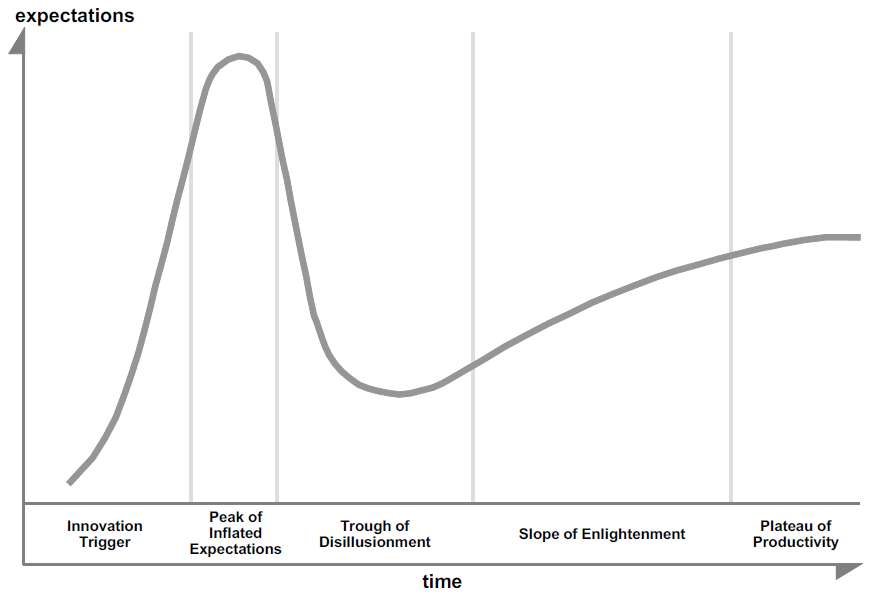
\includegraphics[width=0.9\linewidth]{abbildungen/ghc}
	\caption{Gartner Hype Cycle}
	\label{fig:ghc}
\end{figure}

Deshalb werden die dort aufgeführten Technologien der neusten Ausgabe als Grundlage für den Trendvergleich verwendet. Die letzte Publikation des 
"`Gartner Hype Cycle for Emerging Technologies"' ist im Juli 2017 erschienen und beinhaltet folgende chronologisch sortierte Technologien im Abschnitt "`Peak of Inflated Expectations"':\footcite[Vgl.][S.34-55]{Walker2017}
\begin{enumerate}
	\label{emtech}
	\item Augmented Data Discovery
	\item Edge Computing
	\item Smart Robots
	\item IoT Platform
	\item Virtual Assistants
	\item Connected Home
	\item Deep Learning
	\item Machine Learning
	\item Autonomous Vehicles
	\item Nanotube Electronics
	\item Cognitive Computing
	\item Blockchain
	\item Commercial UAVs (Drones)
\end{enumerate}

Für die Suche dieser Technologien werden zunächst einmal folgende Datenbanken für wissenschaftliche Literatur durchsucht:
\begin{enumerate}
	\item \url{http://ieeexplore.ieee.org/Xplore/home.jsp}
	\item \url{http://dl.acm.org}
	\item \url{http://ipscience.thomsonreuters.com/product/web-of-science}
\end{enumerate}

Falls die Menge an Ergebnissen nicht ausreichen sollte, wird folgende Datenbank zusätzlich hinzugenommen:

\url{http://www.sciencedirect.com}

Die Suchbegriffe werden gegebenenfalls erweitert, falls sie in der wissenschaftlichen Literatur anders verwendet werden.

Anhand der Suchergebnisse wird jeder Technologie eine Matrix mit Suchmaschine, Jahr und Anzahl an Treffern zugeordnet.
Der Betrachtungszeitraum für die Suche erstreckt sich über das Vorjahr des ersten Erscheinens einer der Technologien aus Liste \ref{emtech} im Abschnitt "`Peak of Inflated Expectations"' des "`Gartner Hype Cycle"' bis zum aktuellen Jahr. Das heißt, dass für die Ermittlung des Startjahres alle Hype Cycles der vergangenen Jahre in die Betrachtung einfließen, so lange mindestens eine der aktuellen Technologien im Abschnitt "`Peak of Inflated Expectations"' darin enthalten ist.

Alternativ kann das Erscheinen im Abschnitt "`Innovation Trigger"' als Startzeitpunkt gewählt werden.

Die ermittelte Verteilung der Mengen wird anschließend zunächst pro Suchmaschine und dann kumuliert betrachtet. Die dabei entstandene Kurve der Trefferanzahl über die Zeit wird dazu verwendet, die im Abschnitt "`Peak of Inflated Expectations"' erschienenen Technologien hinsichtlich des Trendverlauf gegenüberzustellen.

\section{Vorläufige Gliederung}
Die Planung der Gliederung wird für 40 Seiten ausgelegt.

\begin{enumerate}
	\item Einleitung (4 Seiten)
	\begin{enumerate}
		\item Ausgangssituation
		\item Motivation
		\item Zielsetzung
		\item Initiale Hypothesen
		\item Vorgehen bei der Literaturrecherche
		\item Methodik der Analyse
	\end{enumerate}
	\item Technologietrends in der praktizierenden Wirtschaft (6 Seiten)
	\begin{enumerate}
		\item Sicht auf Technologien
		\item Einflussfaktoren für Technologietrends
		\item Informationsquellen von Unternehmern
		\item Gartner's Hype Cycle for Emerging Technologies
		\item Schnittpunkte zur akademischen Forschung
	\end{enumerate}
	\item Technologietrends in der akademischen Forschung (4 Seiten)
	\begin{enumerate}
		\item Wissenschaftliche Journals
		\item Zweck von wissenschaftlichen Artikeln
		\item Schnittpunkte zur praktizierenden Wirtschaft
	\end{enumerate}
	\item Methodische Vorgehensweise (7 Seiten)
	\begin{enumerate}
		\item Datenquellen
		\item Beschaffung der Daten
		\item Operationalisierung der Daten
		\item Methodik der Analyse
	\end{enumerate}
	\item Auswertung der Untersuchung (12 Seiten)
	\begin{enumerate}
		\item Trendverlauf im Hype Cyle
		\item Trendverlauf in akademischer Forschung
		\item Gegenüberstellung der Ergebnisse
	\end{enumerate}
	\item Diskussion der Ergebnisse (5 Seiten)
	\item Fazit und Ausblick (2 Seite)
\end{enumerate}

\section{Zeitplan}
\begin{tabular}{|c|c|c|c|}
	\hline 
	Ziel & Startdatum & Enddatum & Dauer \\ 
	\hline 
	Besprechung Exposé & 05.03.2018 & 29.03.2018 & 1 Tag \\ 
	\hline 
	Anmeldung Thesis & 02.04.2018 & 13.04.2018 & 1 Tag \\ 
	\hline 
	Ersterstellung Thesis & 14.04.2018 & 24.06.2018 & 10 Wochen \\ 
	\hline 
	Korrektur & 24.06.2018 & 01.07.2017 & 1 Woche \\ 
	\hline 
	Abgabe & 13.07.2018 & 13.07.2018 & 1 Tag \\ 
	\hline 
\end{tabular} 

\section{Literaturliste}
Das Ergebnis der bisherigen Literaturrecherche ist diesem Dokument als Datei im Text-Format angefügt.
Das endgültige Literaturverzeichnis der Thesis wird im APA-Stil der 6. Edition erstellt.